\documentclass[10pt,a4paper,titlepage]{book}
\usepackage[utf8]{inputenc}
\usepackage{amsmath}
\usepackage{amsfonts}
\usepackage{amssymb}
\usepackage{graphicx}
\usepackage[colorlinks=true,linkcolor=blue]{hyperref}
\usepackage[left=2cm,right=2cm,top=2cm,bottom=2cm]{geometry}
\usepackage[font=small,labelfont=bf]{caption}
\usepackage{times}
\usepackage{parskip}
\usepackage{enumitem}
\setlist{noitemsep}


\begin{document}

\begin{titlepage}
	\centering
	{\scshape\LARGE Spatial Transcriptomics Viewer v0.6.3 User Manual\par}
	\vspace{1cm}
	{\Large Jose Fernandez Navarro\\ Alexander Stuckey\par}
	\vspace{1cm}
	{\today\par}
	\vspace{1cm}
	\href{mailto:alexander.stuckey@scilifelab.se}{alexander.stuckey@scilifelab.se}

\end{titlepage}

\pagenumbering{Roman}

\subsection*{Preface}
The Spatial Transcriptomics viewer (ST viewer) is a desktop application that allows users to securely access and visualize spatially distributed gene expression profile data with their respective tissue image. At the same time it allows users to analyze the data directly, or export it for their own analyses. The application can obtain the data from a secured server (configuration files will need to be updated for this) and/or from local files.


For installation instructions, please see the README.md file. This file describes the install instructions on Windows, OSX and Linux.

%\raggedbottom

%\clearpage
\tableofcontents
\raggedbottom
\clearpage
\listoffigures
\pagenumbering{arabic}

\chapter{Introduction}
\section{User Interface}
 When running the spatial transcriptomics viewer for the first time, you will be presented with an interface as shown in figure \ref{fig:default_view}. If the viewer has been configured to access datasets through the ST API then the login window will be shown, otherwise it will not be shown.
\begin{figure}[h]
	\centering
	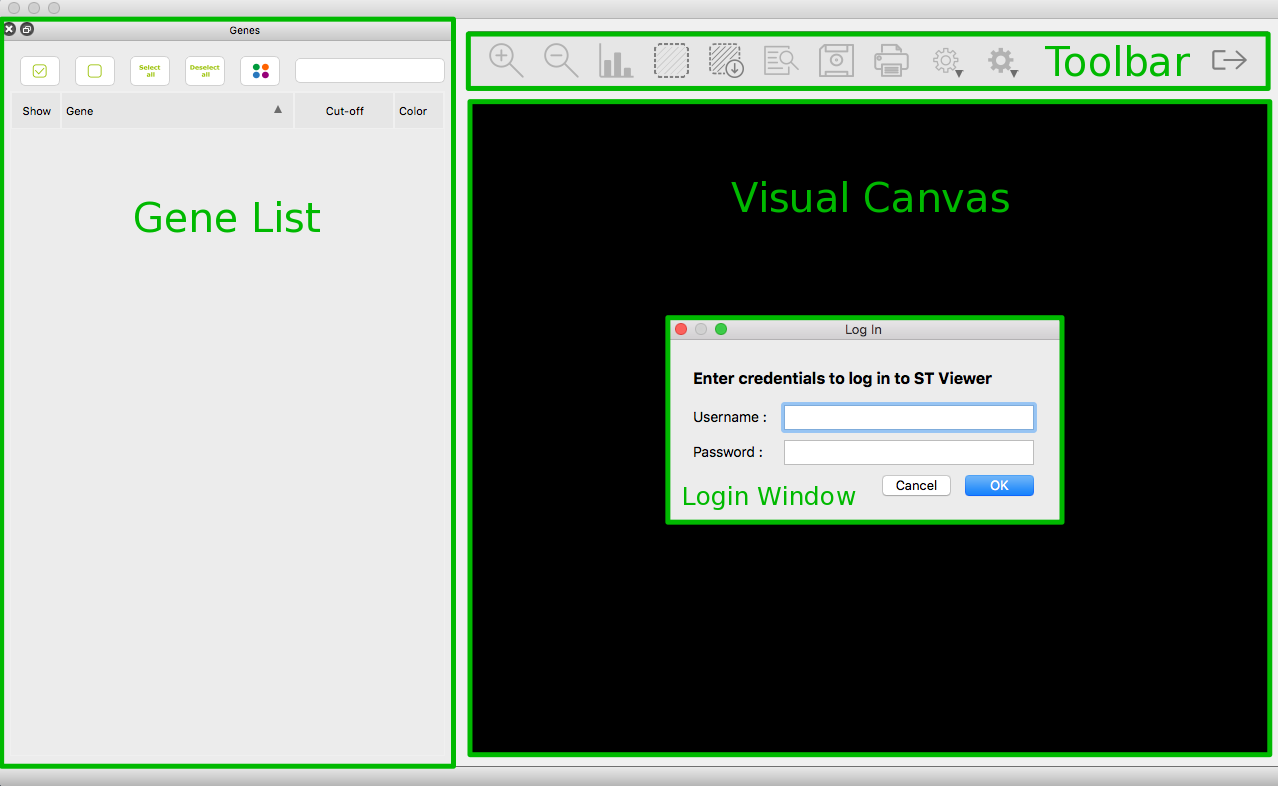
\includegraphics[width=0.9\linewidth]{./Pictures/default_logged_out_labelled}
	\caption[The spatial transcriptomics viewer default interface]{The default interface presented when the ST viewer is run for the first time. The elements present are the gene list window on the left, the toolbar in the top right, the visual canvas on the right, and optionally the log in window (if the viewer is configured to access datasets through the ST API).}
	\label{fig:default_view}

\end{figure}

Once you have logged in (if applicable), your user name will be displayed in the toolbar, as shown in figure \ref{fig:user_name}.
\begin{figure}[h]
	\centering
	
\includegraphics[width=0.9\linewidth]{./Pictures/logged_in}
	\caption{Toolbar showing username after logging in.}
	\label{fig:user_name}
\end{figure}

There are two other main windows in the ST viewer, datasets and selections. They can both be accessed from the views menu by clicking views $\rightarrow$ datasets and views $\rightarrow$ selections.
The datasets window shows all the datasets that you have access to. There is a search box that can be used to find a keyword in the dataset names to narrow down the list of datasets (see figure \ref{fig:datasets_view}). There are five buttons to the right of the dataset search box (labelled 1 --- 5). They are:
\begin{enumerate}
\item Import dataset from file (local file on your computer)
\item Open selected dataset (for datasets stored in the database)
\item Edit selected dataset (change name, add comments)
\item Delete selected dataset
\item Refresh list of datasets
\end{enumerate}

The datasets displayed in the dataset view can also be sorted by each column (e.g. name or species).
\begin{figure}[h]
	\centering
	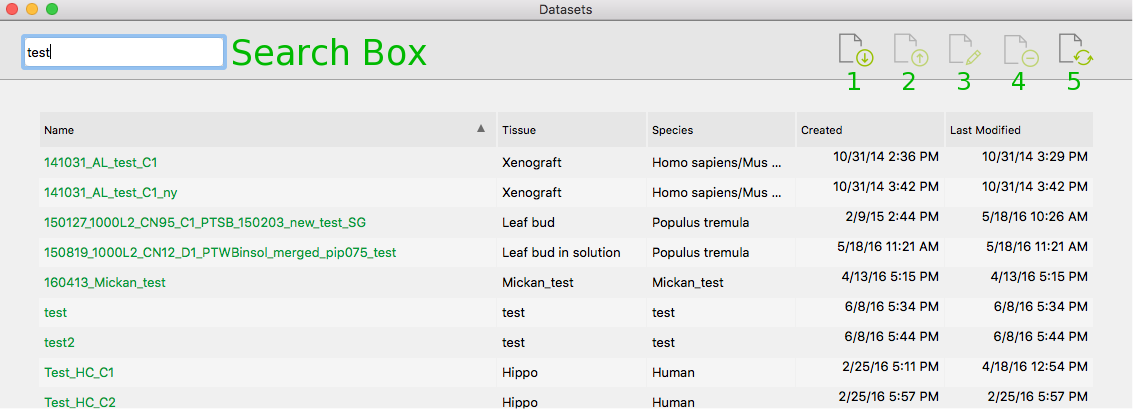
\includegraphics[width=0.9\linewidth]{./Pictures/datasets}
	\caption[Datasets view.]{Datasets view. The search box is being used to display only the datasets that contain the word "test" in their name.}
	\label{fig:datasets_view}
\end{figure}

The selection view will be discussed further in {\LARGE a following chapter}.


{ \textbf Note:} 
Each dataset is associated with a substantial amount of data, which will be accessed after a dataset has been selected and opened. As such the transition between the views might require a few moments. It is worth noting that the data is cached, which implies that once it is downloaded, the next time the same dataset will open much quicker. This does not apply if the dataset is updated in the cloud in the meantime.


When a dataset is loaded, the gene list will populate with the list of all genes that are associated with the current dataset, and the visual canvas will display the image of the tissue section (see figure \ref{fig:default_loaded_data}). 
\begin{figure}[h]
	\centering
	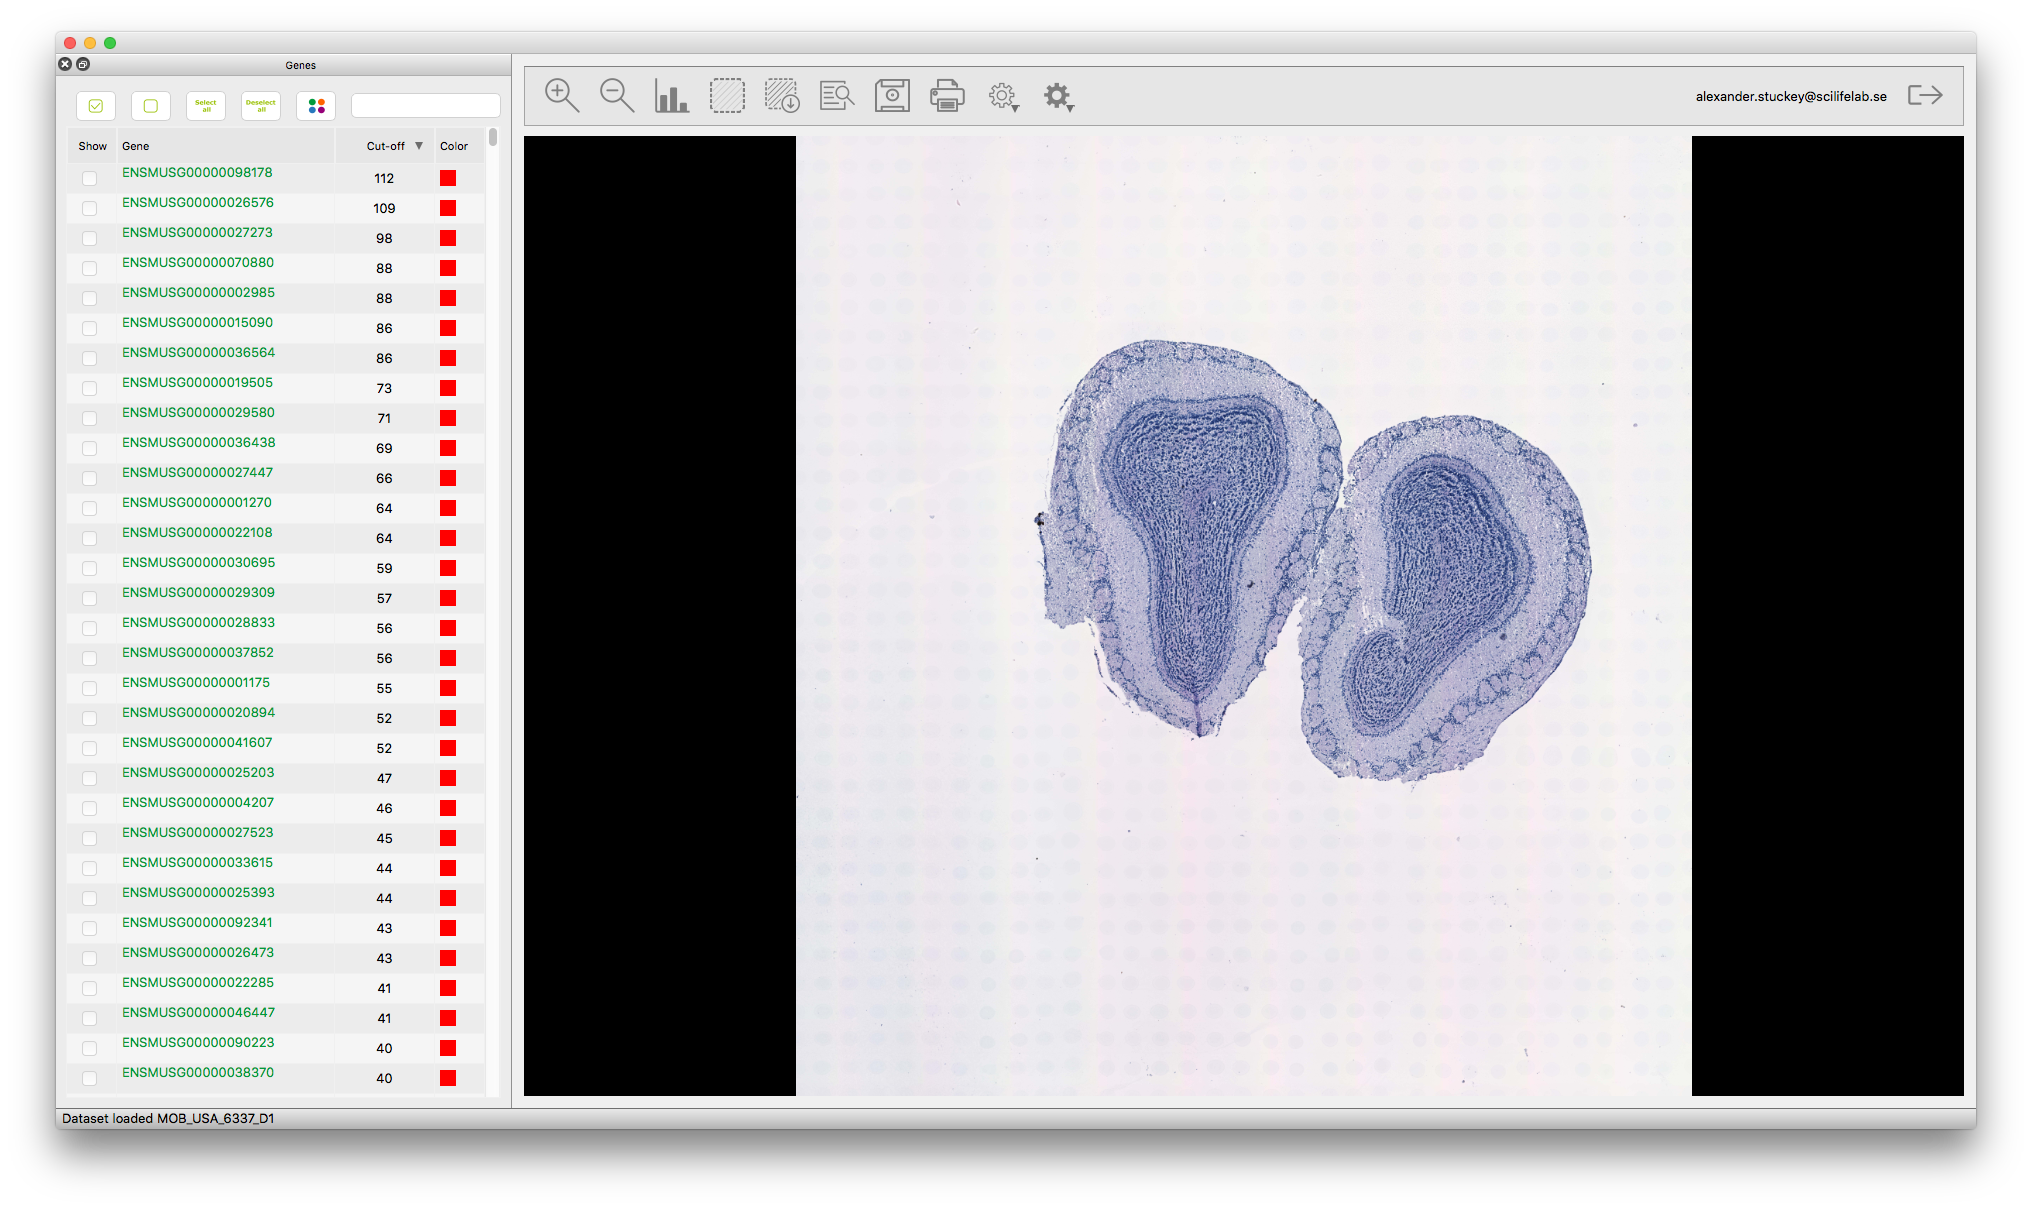
\includegraphics[width=0.9\linewidth]{./Pictures/default_dataset_loaded}
	\caption[Default view after loading a dataset]{The default view after loading a dataset. The gene list is populated by all the genes in the data, and an image of the tissue section is presented on the visual canvas.}
	\label{fig:default_loaded_data}
\end{figure}

The gene list is headed by five buttons and a text box. The buttons are, in order:
\begin{enumerate}
\item	Show selected
\item	Hide selected
\item	Select all
\item	Deselect all
\item	Set colour
\item	Search box
\end{enumerate}

The text box enables you to search the list of genes for genes that are of interest. Shown genes are marked with a checkmark in the box to the left of the gene name / ensemble ID. Selected genes have their names highlighted in orange instead of green, and have a darker grey background. Note that shown genes and selected genes may differ (as seen in figure \ref{fig:gene_list}). The colour column allows you to choose custom colours for single genes or groups of genes, in order to increase visual clarity. The gene list can also be sorted by gene name and cut-off value.

\begin{figure}[h]
	\centering
	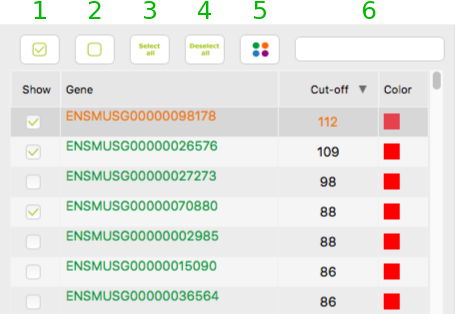
\includegraphics[scale=0.7]{./Pictures/gene_list}
	\caption[Gene List]{Gene list for the current dataset, sorted by cut-off value.}
	\label{fig:gene_list}
\end{figure}

When a dataset is loaded into the viewer the buttons above the visual canvas become active (figure \ref{fig:toolbar_data_loaded}). The buttons on the toolbar are:
\begin{enumerate}
\item	Zoom in
\item	Zoom out
\item	Feature distribution histograms
\item	Selection mode toggle
\item	Create selection object
\item	Feature selection by regular expression
\item	Save a picture of the visual canvas
\item	Print a picture of the visual canvas
\item	Gene display configuration
\item	Visual canvas options
\item	Logout button
\end{enumerate}

\begin{figure}[h]
	\centering
	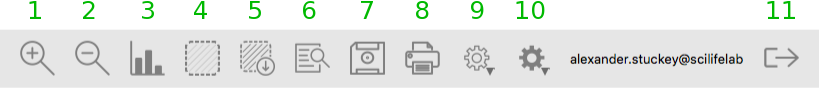
\includegraphics[width=0.9\linewidth]{./Pictures/toolbar_data_loaded}
	\caption{The toolbar when a dataset is loaded.}
	\label{fig:toolbar_data_loaded}
\end{figure}

The gene display configuration is shown in figure \ref{fig:gene_display_config}. From top to bottom, the options are:\\
\textbf{Show Grid} toggles the display of the original array and its border simplified to $5*5$ features per square.\\
\textbf{Show Genes} toggles the display of the currently selected genes.\\
\textbf{Choose Colour Grid} opens a menu to change the colour of the displayed array grid.\\


\textbf{\textit{Gene Display Modes}}\\


In \textbf{Normal Mode} the selected genes in each feature are treated independently. When multiple genes are selected, the final colour of the feature will be a mix of the different colours of the selected genes. In normal mode, the threshold setting treats the genes in each feature separately. Therefore, the threshold can hide some of the selected genes in a feature, or even all the genes in a feature. In all cases, the final colour of the feature will be adjusted accordingly.

In \textbf{Dynamic Range Mode} the selected genes in a feature are all treated as one unit (as opposed to normal mode). This means that each feature is treated as a single unit where the level of expression is determined by the combination of all the genes selected in the feature. The final expression is normalised and the alpha channel (the brightness) of the feature is adjusted according  to the normalised final expression of the feature. This way, users can get an idea of the total expression level of a feature compared to all other features. The colour of each feature will be computed in the same way as in the normal mode (it combines the colours of the genes in each feature).
The threshold in dynamic mode affects features as a whole, instead of gene-by-gene as in normal mode. When the threshold is changed the intensity for all the features is re-calculated, as the normalisation factor might have changed.

\textbf{Heatmap Mode} treats genes in a feature in the same manner as the dynamic range mode. Instead of adjusting the brightness of the colour, a new colour is computed for the feature representing the overall level of expression. The low frequencies are blue and represent a low hit count, while the high frequencies are red and represent a high hit count. The heatmap spectrum and threshold levels can be seen on the legend, when the legend is enabled.
The threshold works the same way as in dynamic range mode, when the threshold is changed the colour range and colour of features will be recalculated.

\begin{figure}[h]
	\centering
	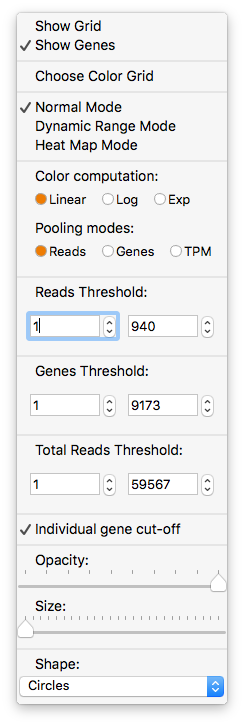
\includegraphics[scale=0.5]{./Pictures/menu_1}
	\caption{Gene display configuration}
	\label{fig:gene_display_config}
\end{figure}

\end{document}